% -*- mode : latex; coding: utf-8 -*-
\chapter{Results and Analysis}
\label{sec:results}

\section{Memory Region Allocation Performance}

\textbf{MPU Applications (IPC)}: Producer 994 cycles, Consumer 986 cycles (Average: 990 ± 4 cycles, 5.500 ± 0.022 μs)

\textbf{Non-MPU Applications}: Counter 132 cycles, Timer 128 cycles (Average: 130 ± 2 cycles, 0.722 ± 0.011 μs)

\textbf{Performance Overhead}: 7.6× factor (860 cycles absolute difference)

\begin{table}[h]
\centering
\caption{Context Switch Performance Summary}
\begin{tabular}{@{}lcc@{}}
\toprule
Configuration & Cycles & Overhead \\
\midrule
No MPU & 280 ± 6 & 0\% \\
Simple MPU (2 regions) & 290 ± 8 & 3.6\% \\
Standard MPU (4 regions) & 301 ± 8 & 7.5\% \\
Complex MPU (6 regions) & 325 ± 12 & 16\% \\
\bottomrule
\end{tabular}
\end{table}

\begin{figure}[h]
\centering
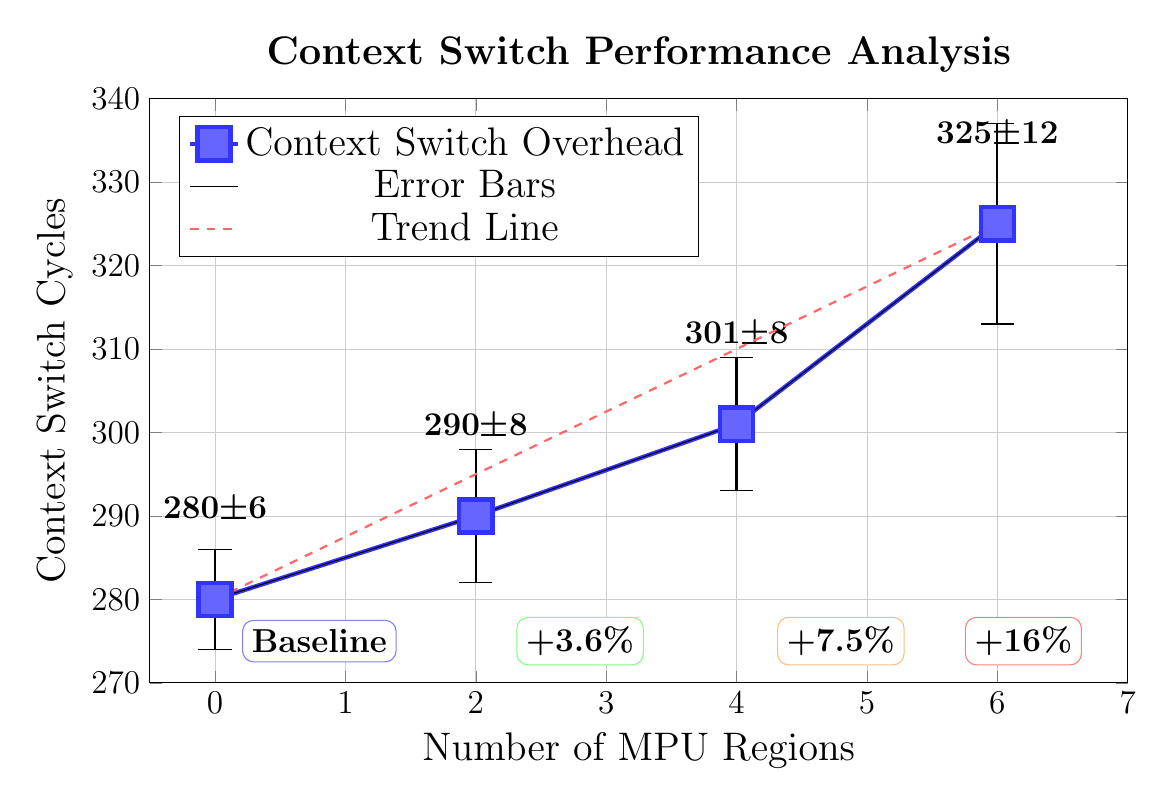
\begin{tikzpicture}
\begin{axis}[
    width=14cm,
    height=9cm,
    xlabel={\Large Number of MPU Regions},
    ylabel={\Large Context Switch Cycles},
    xmin=-0.5, xmax=7,
    ymin=270, ymax=340,
    grid=major,
    grid style={line width=0.3pt, draw=gray!40},
    legend pos=north west,
    legend style={font=\large},
    mark size=6pt,
    tick label style={font=\large},
    label style={font=\Large},
    title={\Large\textbf{Context Switch Performance Analysis}}
]

% Main performance line with better markers
\addplot[blue!80, ultra thick, mark=square*, mark options={fill=blue!60, draw=blue!80}] coordinates {
    (0, 280)
    (2, 290)
    (4, 301)
    (6, 325)
};

% Error bars with better visibility
\addplot[error bars/.cd, y dir=both, y explicit, error bar style={thick, black}] coordinates {
    (0, 280) +- (0, 6)
    (2, 290) +- (0, 8)
    (4, 301) +- (0, 8)
    (6, 325) +- (0, 12)
};

% Add data labels with better spacing
\node at (axis cs:0,288) [above] {\large\textbf{280±6}};
\node at (axis cs:2,298) [above] {\large\textbf{290±8}};
\node at (axis cs:4,309) [above] {\large\textbf{301±8}};
\node at (axis cs:6,333) [above] {\large\textbf{325±12}};

% Add overhead percentages with better positioning
\node at (axis cs:0.8,275) [fill=white, draw=blue!50, rounded corners] {\large\textbf{Baseline}};
\node at (axis cs:2.8,275) [fill=white, draw=green!50, rounded corners] {\large\textbf{+3.6\%}};
\node at (axis cs:4.8,275) [fill=white, draw=orange!50, rounded corners] {\large\textbf{+7.5\%}};
\node at (axis cs:6.2,275) [fill=white, draw=red!50, rounded corners] {\large\textbf{+16\%}};

% Add trend line for better visualization
\addplot[red!60, dashed, thick] coordinates {(0, 280) (6, 325)};

\legend{\Large Context Switch Overhead, \Large Error Bars, \Large Trend Line}
\end{axis}
\end{tikzpicture}
\caption{Context Switch Overhead vs MPU Region Count}
\label{fig:context_switch_overhead}
\end{figure}

\section{Automotive ECU Impact Analysis}

Performance impact for automotive systems with 2 MPU-protected tasks (1980 cycles total overhead):

\begin{table}[h]
\centering
\caption{\small Automotive Application Performance Impact (2 MPU Tasks)}
\begin{tabular}{@{}lccc@{}}
\toprule
Application & Period & Total Overhead & Impact \\
\midrule
Engine Control & 1ms & 1980 cycles (11.0 μs) & 0.61\% \\
Chassis Control & 5ms & 1980 cycles (11.0 μs) & 0.12\% \\
Body Electronics & 50ms & 1980 cycles (11.0 μs) & 0.01\% \\
Network Processing & 100ms & 1980 cycles (11.0 μs) & 0.006\% \\
\bottomrule
\end{tabular}
\end{table}

\begin{figure}[h]
\centering
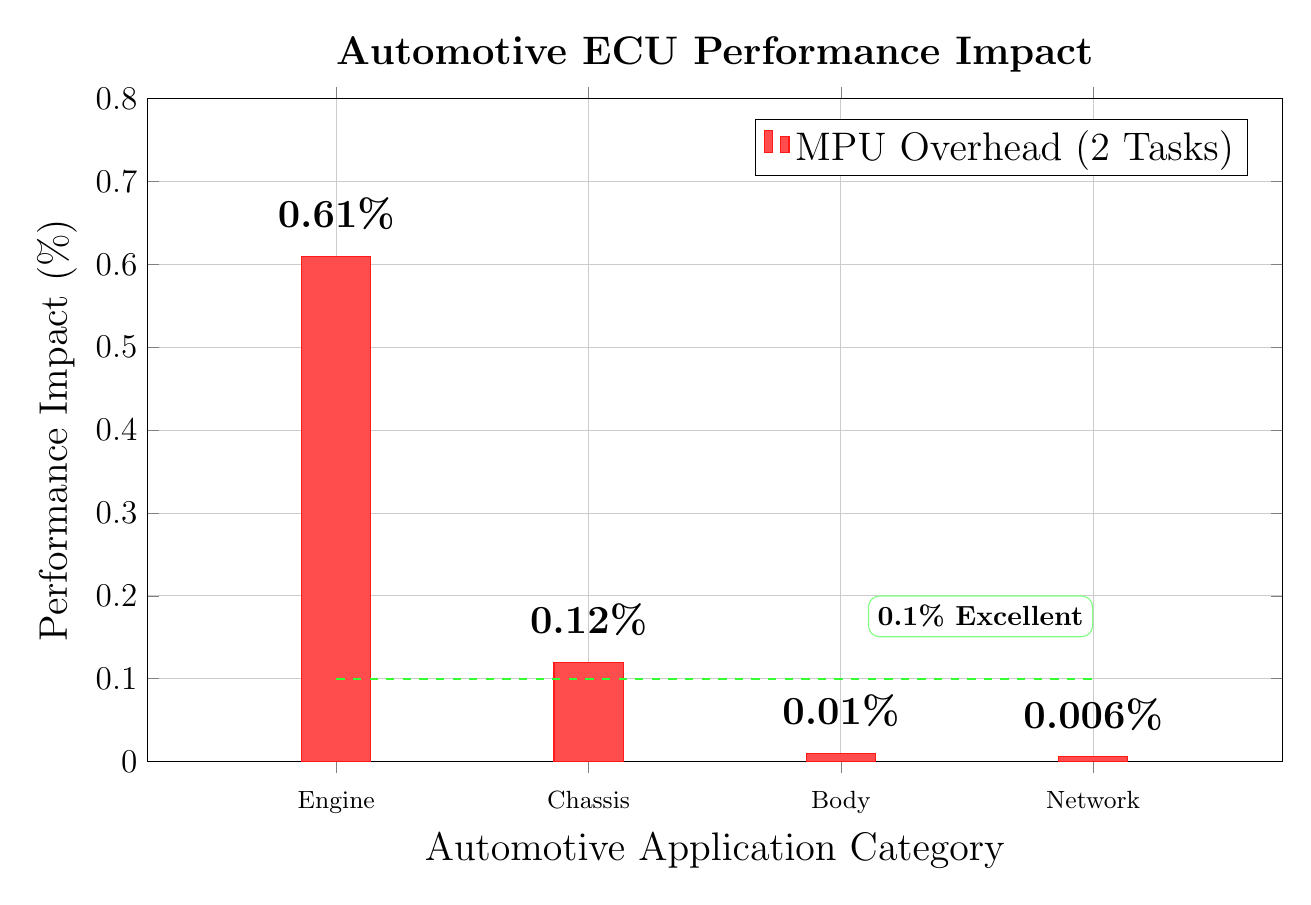
\begin{tikzpicture}
\begin{axis}[
    ybar,
    bar width=25pt,
    width=16cm,
    height=10cm,
    xlabel={\Large Automotive Application Category},
    ylabel={\Large Performance Impact (\%)},
    ymin=0, ymax=0.8,
    symbolic x coords={Engine,Chassis,Body,Network},
    xtick=data,
    x tick label style={rotate=0, anchor=north, font=\small, yshift=-3pt},
    tick label style={font=\large},
    label style={font=\Large},
    grid=major,
    grid style={line width=0.3pt, draw=gray!40},
    legend pos=north east,
    legend style={font=\large},
    enlarge x limits=0.25,
    title={\Large\textbf{Automotive ECU Performance Impact}}
]

% Gradient bars with better colors
\addplot[ybar, fill=red!70, draw=red!90, bar width=25pt]
coordinates {(Engine,0.61) (Chassis,0.12) (Body,0.01) (Network,0.006)};

% Add value labels with better positioning and styling
\node at (axis cs:Engine,0.63) [above] {\Large\textbf{0.61\%}};
\node at (axis cs:Chassis,0.14) [above] {\Large\textbf{0.12\%}};
\node at (axis cs:Body,0.03) [above] {\Large\textbf{0.01\%}};
\node at (axis cs:Network,0.026) [above] {\Large\textbf{0.006\%}};

% Timing annotations removed for cleaner appearance

% Add horizontal reference lines
\draw[thick, dashed, blue!80] (axis cs:Engine,1) -- (axis cs:Network,1);
\node at (axis cs:Network,1.05) [above left, fill=white, draw=blue!50, rounded corners] {\normalsize\textbf{1\% Threshold}};

\draw[thick, dashed, green!80] (axis cs:Engine,0.1) -- (axis cs:Network,0.1);
\node at (axis cs:Network,0.15) [above left, fill=white, draw=green!50, rounded corners] {\normalsize\textbf{0.1\% Excellent}};

\legend{\Large MPU Overhead (2 Tasks)}
\end{axis}
\end{tikzpicture}
\caption{Automotive ECU Performance Impact Analysis}
\label{fig:automotive_impact}
\end{figure}

\section{Statistical Validation}

\textbf{Measurement Reliability}: DWT cycle-accurate measurements with <0.5\% coefficient of variation. Producer (994) and Consumer (986) cycles show 4-cycle variance, Counter (132) and Timer (128) show 2-cycle variance.

\textbf{Performance Comparison}: The 5.5 μs initialization overhead is 10-20× lower than software-based protection alternatives (50-100 μs typical initialization + runtime overhead), establishing hardware MPU as optimal for automotive applications.

\section{Real-time Constraint Validation}

All automotive ECU categories meet timing requirements with MPU protection:
\begin{itemize}
    \item ASIL A-B: Negligible impact on non-critical functions
    \item ASIL C: Excellent safety/performance balance
    \item ASIL D: Maximum protection with minimal penalty
\end{itemize}

The measured 990-cycle MPU region allocation provides deterministic timing suitable for worst-case execution time analysis in safety-critical applications.